\documentclass[border=3pt]{standalone}
% Preâmbulo compartilhado pelos diagramas TikZ da aula 12 (Mapeamento por Grade de Ocupação)
\usepackage[T1]{fontenc}
\usepackage[utf8]{inputenc}
\usepackage{lmodern}
\usepackage{amsmath}
\usepackage{xcolor}
\usepackage{tikz}
\usetikzlibrary{arrows.meta,angles,quotes,decorations.pathmorphing,calc,
                positioning,shapes.geometric,shapes.misc,backgrounds,fit,
                math}

% Paleta (mesma dos SVGs originais)
\definecolor{dblue}{HTML}{2A5B8C}
\definecolor{dorange}{HTML}{B3541E}
\definecolor{dgreen}{HTML}{4A7C59}
\definecolor{dred}{HTML}{9C4B4B}
\definecolor{dcream}{HTML}{F4F1EA}
\definecolor{dshade}{HTML}{DDD7C9}

% Função gaussiana (não normalizada por padrão de escala visual)
\pgfmathdeclarefunction{gauss}{3}{%
  \pgfmathparse{1/(#3*sqrt(2*pi))*exp(-((#1-#2)^2)/(2*#3^2))}%
}

% Estilos comuns (prefixo d... para não colidir com chaves internas do pgf)
\tikzset{
  >={Stealth[length=2mm]},
  dguide/.style={gray!55, dashed, line width=0.4pt},
  daxis/.style={gray!60, line width=0.7pt, ->},
  dbody/.style={fill=black!3, draw=black!80, line width=1pt},
  dacc/.style={draw=dblue, line width=1pt},
  dlbl/.style={black!55, font=\small},
  dsub/.style={black!45, font=\footnotesize},
  dstate/.style={circle, draw=black!80, fill=dcream, line width=1pt,
                 minimum size=17mm, font=\large, inner sep=1pt},
  dobs/.style={circle, draw=black!80, fill=dshade, line width=1pt,
               minimum size=14mm, font=\large, inner sep=1pt},
  dbox/.style={rounded corners=2pt, draw=black!80, fill=dcream, line width=1pt,
               align=center, inner sep=6pt},
  dop/.style={circle, draw=black!80, fill=white, line width=1pt,
              minimum size=6mm, inner sep=0pt, font=\small},
  dtrans/.style={->, dblue, line width=1pt},
  dmeas/.style={->, dorange, line width=1pt},
  dcurve/.style={line width=1pt, dblue},
  dcurveb/.style={line width=1.4pt, dorange},
}

\begin{document}
\hyphenpenalty=10000 \exhyphenpenalty=10000 \tolerance=9999 \emergencystretch=3em
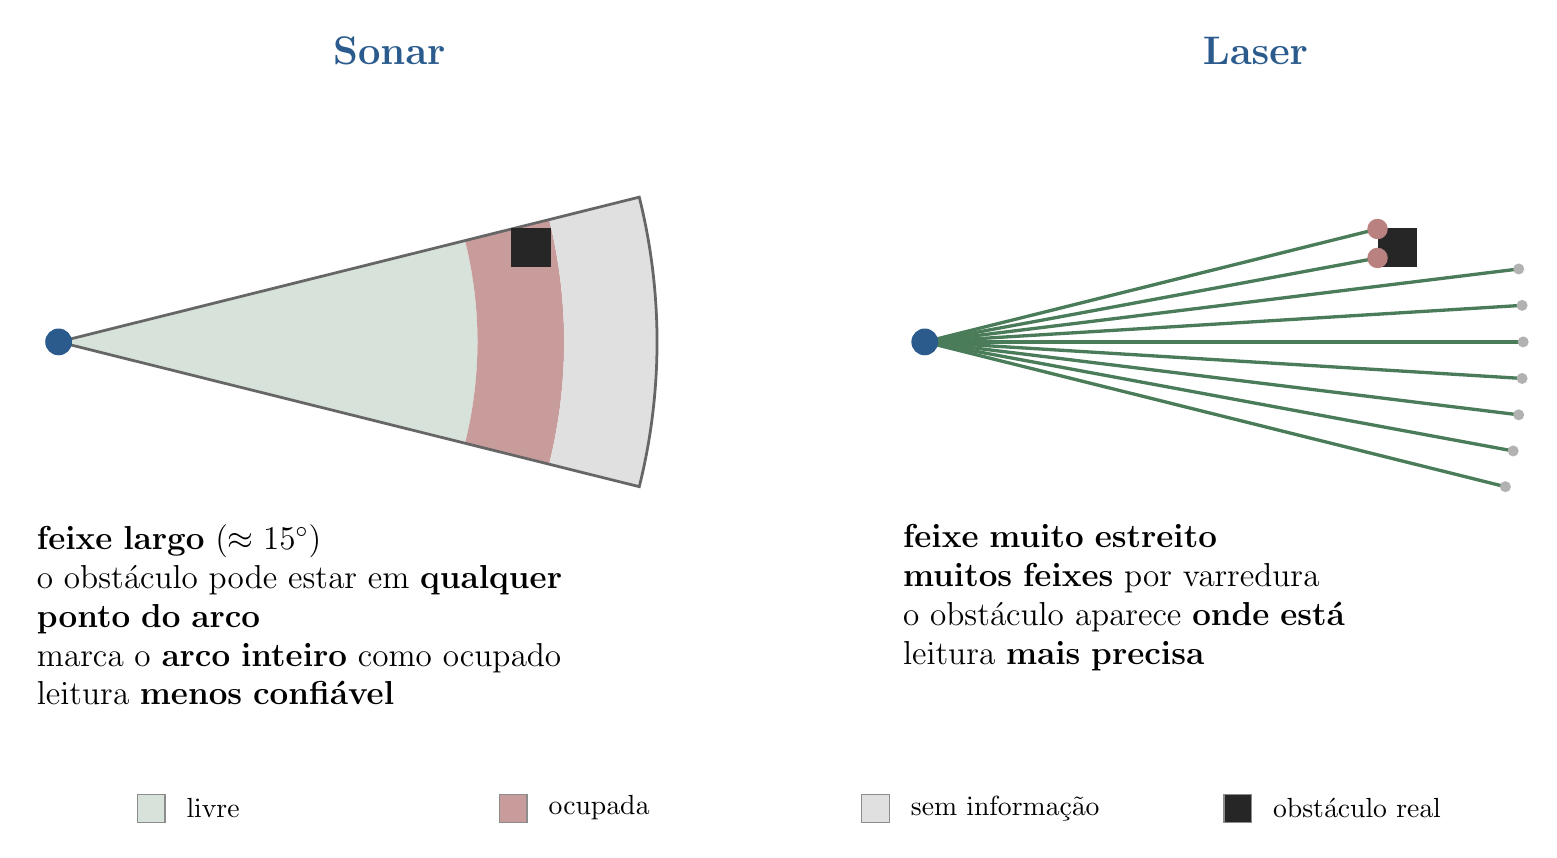
\begin{tikzpicture}[x=1cm,y=1cm]
\node[font=\Large\bfseries, dblue] at (4.2,3.7) {Sonar};
  \fill[dgreen!22] (0,0) -- (-14.0:5.32) arc(-14.0:14.0:5.32) -- cycle;
  \fill[dred!55] (-14.0:5.32) arc(-14.0:14.0:5.32) -- (14.0:6.42) arc(14.0:-14.0:6.42) -- cycle;
  \fill[black!12] (-14.0:6.42) arc(-14.0:14.0:6.42) -- (14.0:7.6) arc(14.0:-14.0:7.6) -- cycle;
  \draw[black!60, line width=1pt] (0,0) -- (-14.0:7.6) arc(-14.0:14.0:7.6) -- cycle;
  \fill[black!85] (5.75,0.95) rectangle +(0.5,0.5);
  \fill[dblue] (0,0) circle (0.17);
  \begin{scope}[shift={(11.0,0)}]
  \node[font=\Large\bfseries, dblue] at (4.2,3.7) {Laser};
  \fill[black!85] (5.75,0.95) rectangle +(0.5,0.5);
  \draw[dgreen, line width=1.2pt] (0,0) -- (7.374,-1.839);
  \fill[black!30] (7.374,-1.839) circle (0.07);
  \draw[dgreen, line width=1.2pt] (0,0) -- (7.473,-1.385);
  \fill[black!30] (7.473,-1.385) circle (0.07);
  \draw[dgreen, line width=1.2pt] (0,0) -- (7.543,-0.926);
  \fill[black!30] (7.543,-0.926) circle (0.07);
  \draw[dgreen, line width=1.2pt] (0,0) -- (7.586,-0.464);
  \fill[black!30] (7.586,-0.464) circle (0.07);
  \draw[dgreen, line width=1.2pt] (0,0) -- (7.6,0.0);
  \fill[black!30] (7.6,0.0) circle (0.07);
  \draw[dgreen, line width=1.2pt] (0,0) -- (7.586,0.464);
  \fill[black!30] (7.586,0.464) circle (0.07);
  \draw[dgreen, line width=1.2pt] (0,0) -- (7.543,0.926);
  \fill[black!30] (7.543,0.926) circle (0.07);
  \draw[dgreen, line width=1.2pt] (0,0) -- (5.75,1.066);
  \fill[dred!70] (5.75,1.066) circle (0.13);
  \draw[dgreen, line width=1.2pt] (0,0) -- (5.75,1.434);
  \fill[dred!70] (5.75,1.434) circle (0.13);
  \fill[dblue] (0,0) circle (0.17);
  \end{scope}
  \node[font=\large, text width=7.8cm, align=left, anchor=north west] at (-0.4,-2.2) {\textbf{feixe largo} ($\approx 15^\circ$)\\ o obstáculo pode estar em \textbf{qualquer ponto do arco}\\ marca o \textbf{arco inteiro} como ocupado\\ leitura \textbf{menos confiável}};
  \node[font=\large, text width=7.8cm, align=left, anchor=north west] at (10.6,-2.2) {\textbf{feixe muito estreito}\\ \textbf{muitos feixes} por varredura\\ o obstáculo aparece \textbf{onde está}\\ leitura \textbf{mais precisa}};
  \fill[dgreen!22] (1.0,-6.1) rectangle +(0.35,0.35);
  \draw[black!45, line width=0.5pt] (1.0,-6.1) rectangle +(0.35,0.35);
  \node[font=\normalsize, anchor=west] at (1.5,-5.92) {livre};
  \fill[dred!55] (5.6,-6.1) rectangle +(0.35,0.35);
  \draw[black!45, line width=0.5pt] (5.6,-6.1) rectangle +(0.35,0.35);
  \node[font=\normalsize, anchor=west] at (6.1,-5.92) {ocupada};
  \fill[black!12] (10.2,-6.1) rectangle +(0.35,0.35);
  \draw[black!45, line width=0.5pt] (10.2,-6.1) rectangle +(0.35,0.35);
  \node[font=\normalsize, anchor=west] at (10.7,-5.92) {sem informação};
  \fill[black!85] (14.799999999999999,-6.1) rectangle +(0.35,0.35);
  \draw[black!45, line width=0.5pt] (14.799999999999999,-6.1) rectangle +(0.35,0.35);
  \node[font=\normalsize, anchor=west] at (15.3,-5.92) {obstáculo real};
\end{tikzpicture}
\end{document}
